\subsection{Clifford Circuits}

\begin{definition}
A \term{Clifford circuit} is a quantum circuit made of \term{Clifford gates}:\footnote{This is not the typical formal definition of Clifford circuits. However, we will soon show that this definition is equivalent to the usual one, i.e. as the circuits that normalize the Pauli group.}
\begin{equation}
\begin{alignedat}{3}
    \CNOT := \begin{ZX}
        \rar & \zxZ{} \dar \rar & \\
        \rar & \zxX{} \rar      &
    \end{ZX}, \quad 
    &\Had := \begin{ZX}
        \rar & \zxH{} \rar & 
    \end{ZX} = \begin{ZX}
             &                          & \zxZ{-\frac{\pi}{2}} \dar & & \\
        \rar & \zxZ{\frac{\pi}{2}} \rar & \zxX{} \rar & \zxZ{\frac{\pi}{2}} \rar &
    \end{ZX}, \quad 
    &\Sgate := \begin{ZX}
        \rar & \zxZ{\frac{\pi}{2}} \rar &  
    \end{ZX}.
\end{alignedat}
\end{equation}
Furthermore, let $\Had$ and $\Sgate$ be known as the \term{local Clifford gates}.
\end{definition}

\begin{definition}
A \term{Clifford ZX diagram} is a ZX diagram made up only of spiders whose phases are multiples of $\tfrac{\pi}{2}$. Furthermore, say a ZX diagram $D$ is \term{unitary} if $\llbracket D \rrbracket = c U$ for some $c \in \C$ and unitary matrix $U$.
\end{definition}

\begin{theorem}
\label{thm:clifford-circuits-are-clifford-diagrams}
Clifford circuits are precisely the unitary Clifford ZX diagrams. That is, every Clifford circuit can be written as a unitary Clifford ZX diagram and vice versa.
\end{theorem}

\begin{proof}[Proof, part 1]
It is clear that any Clifford circuit is a Clifford ZX diagram, since the diagrams of the Clifford gates only involve spiders with phases multiples of $\tfrac{\pi}{2}$. The reverse direction, however, will take more work.
\end{proof}

To show the reverse direction, we construct an algorithm from Chapter 5 of \cite{PQS} that allows us to convert any unitary Clifford ZX diagram into a Clifford circuit.

\begin{definition}
A \term{Hadamard wire} is a wire with a single Hadamard, i.e. \zx{\rar & \zxH{} \rar &}. To further disambiguate this from \zx{\rar & \zxZ{} \rar &}, we may write \zx{\ar[r,hw] & \ar[r,hw] &} in place of \zx{\rar & \zxH{} \rar &}.
\end{definition}

\begin{definition}
A ZX diagram is \term{graph-like} when:
\begin{enumerate}[label=(\alph*)]
    \item Every spider is a Z-spider.
    \item Spiders are only connected via Hadamard edges.
    \item There are no self loops or parallel i.e. duplicate edges.
    \item Every Z-spider is connected to at most one input and at most one output via a regular edge.
    \item Every input and output is connected to a Z-spider.
\end{enumerate}
\end{definition}

\begin{theorem}
\label{thm:zx-to-graph-like}
Every ZX diagram can be efficiently rewritten as a graph-like diagram.
\end{theorem}

\begin{proof}
Let $D$ be an arbitrary ZX diagram. Run the following algorithm:
\begin{enumerate}
    \item Convert all X-spiders to Z-spiders via \zxref{cc}.
    \item Cancel adjacent $\Had$ with \zxref{hh}.
    \item Fuse all connected spiders via \zxref{cc} until this cannot be done.
    \item Remove parallel Hadamard edges via:
\begin{align}
    \begin{ZX}
        \leftManyDots{} \zxZ{\alpha} \ar[r,H,(] \ar[r,H,)] & \zxZ{\beta} \rightManyDots{} 
    \end{ZX}
    \overset{\substack{\zxref{cc} \\ \zxref{f}}}{=}
    \begin{ZX}
        \leftManyHDots{} \zxX{\alpha} \rar & \zxX{} \ar[r,(] \ar[r,)] & \zxZ{} \rar & \zxZ{\beta} \rightManyDots{}
    \end{ZX}
    \overset{\zxref{hf}}{=}
    \begin{ZX}
        \leftManyHDots{} \zxX{\alpha} \rar & \zxX{} & \zxZ{} \rar & \zxZ{\beta} \rightManyDots{}
    \end{ZX}
    \overset{\substack{\zxref{f} \\ \zxref{cc}}}{=}
    \begin{ZX}
        \leftManyDots{} \zxX{\alpha} \rar & \zxZ{\beta} \rightManyDots{}
    \end{ZX}.
\end{align}
    \item Remove self-loops via:
\begin{align}
    \begin{ZX}
        \leftManyDots{} \zxZ{\alpha} \zxLoop{} \rightManyDots{}
    \end{ZX}
    &\overset{\zxref{id}}{=}
    \begin{ZX}
        \leftManyDots{} \zxZ{\alpha} \zxLoop[90][20][Z]{} \rightManyDots{}
    \end{ZX}
    \overset{\zxref{f}}{=}
    \begin{ZX}
        \leftManyDots{} \zxZ{\alpha} \rightManyDots{}
    \end{ZX}, \\
    \begin{ZX}
        \leftManyDots{} \zxZ{\alpha} \zxLoop[90][20][H]{} \rightManyDots{} 
    \end{ZX}
    &\overset{\zxref{f}}{\propto}
    \begin{ZX}
        \leftManyDots{} \zxZ{\alpha+\pi} \zxLoopXPhase{\frac{\pi}{2}} \rightManyDots{} 
    \end{ZX}
    \overset{\substack{\zxref{f} \\ \zxref{hf}}}{\propto}
    \begin{ZX}
        \leftManyDots{} \zxZ{\alpha+\pi} \rightManyDots{} 
    \end{ZX}.
\end{align}
    \item Introduce Z-spiders and Hadamards using \zxref{id} and \zxref{hh} to ensure every input and output is connected to a Z-spider and no Z-spiders are connected to multiple inputs or multiple outputs.
\end{enumerate}
After this, all spiders are Z-spiders. All edges between spiders are Hadamard edges, else the spiders would have been fused together. There is at most one edge between any two spiders, and there are no self-loops. Step 6 ensures (e) is satisfied.
\end{proof}

Note that the above procedure applies to any ZX diagram, not just Clifford ones. As it turns out, when our starting ZX diagram is Clifford, we can simplify the diagram even further. To see how, we introduce the notion of a graph state and some operations on them.

\begin{definition}
\label{def:internal-boundary-spiders}
Say a spider in a ZX diagram is \term{internal} if it is not directly connected to an input or output wire, but it has a connection via other spiders to an input or output wire. Conversely, a spider is a \term{boundary} spider if it is directly connected to an input or output wire.
\end{definition}

\begin{definition}
\label{def:graph-state}
For a simple, undirected graph $G = (V,E)$, the \term{graph state} $\ket{G}$ of $G$ is defined
\begin{align}
    \ket{G} := \prod_{(v,w) \in E} \CZ_{v,w} \ket{+}^{\otimes |V|}.
\end{align}
That is, prepare the $\ket{+}^{\otimes |V|}$ state and apply a $\CZ$ gate between every pair of adjacent vertices in $G$. If $D$ is a ZX diagram and graph state, we write $G(D) = (V,E)$ to refer to the graph. Note that in the ZX Calculus, 
\begin{equation}
\begin{alignedat}{2}
    \ket{+} \propto \begin{ZX}
        \zxZ{} \rar &
    \end{ZX}, \quad
    &\CZ = \begin{ZX}
        \rar & \zxZ{} \ar[d,H] \rar & \\
        \rar & \zxZ{} \rar &
    \end{ZX}.
\end{alignedat}
\end{equation}
\end{definition}

\begin{figure}[H]
\centering
\begin{tabular}{CCC}
    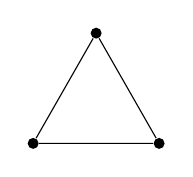
\begin{tikzpicture}[every node/.style={circle,fill,inner sep=1.4pt}]
    \node (a) at (0,0.9) {};
    \node (b) at (-0.8,-0.5) {};
    \node (c) at (0.8,-0.5) {};
    \draw (a)--(b)--(c)--(a);
    \end{tikzpicture}
&
    \begin{ZX}[circuit,mbr=3]
        \zxInput{\ket0} \ar[r] & \zxCross{} \ar[d] \rar & \zxCross{} \ar[dd] \rar & \rar & \\
        \zxInput{\ket0} \ar[r] & \zxCross{} \rar & \rar & \zxCross{} \ar[d] \rar & \\
        \zxInput{\ket0} \ar[r] & \rar & \zxCross{} \rar & \zxCross{} \rar &
    \end{ZX}
&
    \begin{ZX}[mbr=3]
        \zxZ{} \ar[r,hw] & \zxZ{} \ar[d,hw] \rar & \zxZ{} \ar[dd,hw] \rar & \rar & \\
        \zxZ{} \ar[r,hw] & \zxZ{} \rar & \rar & \zxZ{} \ar[d,hw] \rar & \\
        \zxZ{} \ar[r,hw] & \rar & \zxZ{} \rar & \zxZ{} \rar &
    \end{ZX}
\end{tabular}
\caption{The triangle graph and its circuit and ZX graph state.}
\label{fig:triangle-graph}
\end{figure}

\begin{definition}
\label{def:gslc}
A \term{graph state with local Cliffords (GSLC)} is a graph state to which some single-qubit Clifford unitaries have been applied on its outputs.
\end{definition}

\begin{theorem}
\label{thm:clifford-to-gslc}
Every Clifford ZX diagram can be written in GSLC form.
\end{theorem}

To prove Theorem \ref{thm:clifford-to-gslc}, we need to show that all internal spiders in a Clifford ZX diagram in graph-like form can be removed, perhaps by changing the phases of some of the boundary spiders and adding local Cliffords. To do this we need the following graph operations.

\begin{definition}
Let $G$ be a graph and $u \in V(G)$. The \term{local complementation} of $G$ around $u$, written $G \star u$, is the graph obtained by complementing the subgraph induced by the neighbors of $u$. For distinct $v,w \in V(G)$, let $e_{v,w}$ be the edge between them. Then 
\begin{align}
    e_{v,w} \in E(G \star u) \iff \begin{cases}
        e_{v,w} \notin E(G) & \text{if } v,w \in N_G(u), \\
        e_{v,w} \in E(G) & \text{otherwise.}
    \end{cases}
\end{align}
\end{definition}

\begin{lemma}
\label{lemma:zx-local-complement-without-deletion}
Let $D$ be a graph-state ZX diagram, and $u$ some vertex in $G(D)$. Then we can obtain a diagram $D'$ with $G(D') = G(D) \star u$ by applying a $R_X(-\pi/2)$ gate on the spider corresponding to $u$ and $R_Z(\pi/2)$ on all spiders in $N_{G(D)}(u)$. Call this rule \zxlabel{lc}{($lc$)}:
\begin{align}
    \begin{ZX}
        \dar & \dar & \dar & \dar \\
            \zxX{\pm\frac{\pi}{2}} \dar & 
            \zxZ{\mp\frac{\pi}{2}} \ar[dd] &
            \zxZ{\mp\frac{\pi}{2}} \ar[d] &
            \zxZ{\mp\frac{\pi}{2}} \ar[dd] \\
        \zxZ{} \ar[rr,hw] \ar[dr,hw] \ar[drrr,hw] & & \zxZ{} \ar[r,3 dots] \ar[dr,hw] & \\
        u & \zxZ{} & & \zxZ{} \\[\zxNRow]
        & \zxVInputMulti{3}{N(u)} & &
    \end{ZX}
    \overset{\zxref{lc}}{=}
    \begin{ZX}
        \dar & \dar & \dar & \dar \\
        \dar & \ar[dd] & \ar[d] & \ar[dd] \\[\zxSRow]
        \zxZ{} \ar[rr,hw] \ar[dr,hw] \ar[drrr,hw] & & \zxZ{} \ar[r,3 dots] & \\
        u & \zxZ{} \ar[ur,hw] \ar[rr,hw]& & \zxZ{} \\[\zxNRow]
        & \zxVInputMulti{3}{N(u)} & &
    \end{ZX}.
\end{align}
Thus by applying local Cliffords we can local complement a graph state.
\end{lemma}

\begin{proof}
This was originally proved in Theorem 2 of \cite{zx-graph-proofs}. The proof surmounts to a clever decomposition of the H-box as Z and X-spiders, which after some application of the rules in Table \ref{table:zx-rules} gives the desired result.
\end{proof}

\begin{lemma}
\label{lemma:remove-half-pi-from-graph}
The following holds:
\begin{align}
    \begin{ZX}
        & & & \zxZ[label={[yshift=2mm]above:{\star}}]{\pm \frac{\pi}{2}} \ar[drr,hw] \ar[ddr,hw] & \\
        \leftManyDots{} \zxZ{\alpha_1} \ar[urr,hw] & & \cdots & &
        \zxZ{\alpha_n} \rightManyDots{} \\
        & \leftManyDots{} \zxZ{\alpha_2} \ar[uur,hw] & &
        \zxZ{\alpha_{n-1}} \rightManyDots{} &
    \end{ZX} = 
    \begin{ZX}
        \leftManyDots{} \zxZ{\alpha_1 \mp \frac{\pi}{2}} \ar[rrrr,hw,)] \ar[dr,hw] \ar[drrr,hw] & & \cdots & &
        \zxZ{\alpha_n \mp \frac{\pi}{2}} \rightManyDots{} \\
        & \leftManyDots{} \zxZ{\alpha_2 \mp \frac{\pi}{2}} \ar[urrr,hw] \ar[rr,hw] & &
        \zxZ{\alpha_{n-1} \mp \frac{\pi}{2}} \ar[ur,hw] \rightManyDots{} &
    \end{ZX}.
\end{align}
Here, the $\star$ above \zx{\zxZ{\pm \frac{\pi}{2}}} indicates a local complementation at this vertex.
\end{lemma}

\begin{proof}
We provide a proof sketch: Let $u$ denote the vertex we local complement around. First, push out all the phases via \zxref{f} to obtain a graph state where all the vertices are phase-free Z-spiders. Apply local complementation in reverse around $u$. Then $u$ will have \zx{\zxZ{\pm \frac{\pi}{2}} \rar & \zxX{\pm \frac{\pi}{2}} \rar &} = \zx{\zxX{} \rar &} dangling from it. Apply \zxref{cp} to push the \zx{\zxX{} \rar &} through and disconnect $u$. This gives the RHS. For a step-by-step proof, see Appendix B.3 of \cite{zx-clifford-simplification}.
\end{proof}

\begin{definition}
Let $G$ be a graph, $u,v \in V(G)$, and $e_{vw} \in E(G)$. The pivot of $G$ along $uv$, denoted $G \land uv$, is defined as
\begin{align}
    G \land uv := G \star u \star v \star u 
\end{align}
or equivalently
\begin{align}
    G \land uv = G \star v \star u \star v.
\end{align}
\end{definition}

\begin{proof}
This is a standard proof by cases, seen for example in Definition 4.3 of \cite{zx-clifford-simplification}.
\end{proof}

\begin{lemma}
\label{lemma:zx-pivot-without-deleting}
Given a graph $G$, we can pivot around $uv$ for $u,v \in V(G)$ by applying Hadamard on $u$ and $v$ and $Z$ on all vertices in $N_G(u) \cap N_G(v)$, inducing a swap gate between $u$ and $v$.
\end{lemma}

\begin{proof}
The proof is surprisingly involved and can be found in Proposition 3.1 of \cite{zx-pivoting-proof}.
\end{proof}

\begin{lemma}
\label{lemma:remove-pi-from-graph}
The following holds:
\begin{align}
    \begin{ZX}
        \leftManyDots{} \zxZ{\alpha_1} 
            \ar[r,hw] \ar[d,3 vdots] &
        \zxZ[label={[yshift=2mm]above:{\star}}]{j \pi}
            \ar[rr,hw] \ar[dr,hw] \ar[ddr,hw] & &
        \zxZ[label={[yshift=2mm]above:{\star}}]{k \pi}
            \ar[r,hw] \ar[dr,hw] \ar[d,3 vdots] &
        \zxZ{\gamma_1} 
            \rightManyDots{} \\
        \leftManyDots{} \zxZ{\alpha_n} 
            \ar[ur,hw] & &
        \zxZ{\beta_1} 
            \ar[ur,hw] \ar[d, 3 vdots] & & 
        \zxZ{\gamma_o} 
            \rightManyDots{}\\
        & & & \zxZ{\beta_m} 
            \ar[uur,hw] &
    \end{ZX}
    =
    \begin{ZX}
        \leftManyDots{} \zxZ{\alpha_1 + k\pi}
            \ar[rrrr,hw] \ar[rrrrd,hw] \ar[drr,hw] \ar[ddrr,hw] 
            \ar[d,3 vdots] & & & &
        \zxZ{\gamma_1 + j \pi} \ar[d,3 vdots] \rightManyDots{} \\
        \leftManyDots{} \zxZ{\alpha_n + k \pi} 
            \ar[rrrr,hw,)] \ar[rrrru,hw] \ar[rr,hw] \ar[drr,hw] & &
        \zxZ{\beta_1 + (j + k + 1) \pi} 
            \ar[urr,hw] \ar[rr,hw]
            \ar[d, 3 vdots] & & 
        \zxZ{\gamma_o + j \pi} \rightManyDots{}\\
        & & & \zxZ{\beta_m + (j + k + 1) \pi} 
            \ar[uurr,hw] \ar[urr,hw] &
    \end{ZX}.
\end{align}
Note that the vertices $\beta_1, \ldots, \beta_m$ may have other wires, but we suppress them here to reduce clutter.
\end{lemma}

\begin{proof}
We provide a proof sketch: Let $u$ denote the vertex with phase $j \pi$ and $v$ the vertex with phase $k \pi$. First, push out all the phases via \zxref{f} to obtain a graph state where all the vertices are phase-free Z-spiders. Apply pivoting on $uv$. Then $u$ will have \zx{\zxZ{k \pi} \rar & \zxH{} \rar &} dangling from it (note the change from $j$ to $k$ due to the pivoting's swap gate), and similarly for $v$. Apply \zxref{cc} and \zxref{cp} to obtain the RHS after fusing with \zxref{f}. For a step-by-step proof, see Appendix B.3 of \cite{zx-clifford-simplification}.
\end{proof}

\begin{proof}[Proof of Theorem \ref{thm:clifford-to-gslc}]
First note that by Theorem \ref{thm:yanking}, we can topologically morph the inputs of the Clifford circuit to face rightwards, like outputs, and that this has no effect on the operation represented by the diagram. Now, start by converting a Clifford ZX diagram to graph-like form. Apply Lemma \ref{lemma:remove-half-pi-from-graph} amd \ref{lemma:remove-pi-from-graph} to remove all internal spiders from the diagram, perhaps appending local Clifford gates to the output wires. This gives a circuit in GSLC form.
\end{proof}

\begin{lemma}
\label{lemma:zx-lc-graph-lc-form}
The GSLC form of a CLifford ZX diagram may be written as follows:
\begin{align}
    \begin{ZX}
    \rar & \zxGate{LC} \ar[d,3 vdots] \rar &
    \zxZ{} \ar[d,3 vdots] \rightManyHDots{} &
    \leftManyHDots{} \zxZ{} \ar[d,3 vdots] \rar &
    \zxGate{LC} \ar[d,3 vdots] \rar & \\
    \rar & \zxGate{LC} \rar &
    \zxZ{} \rightManyHDots{} &
    \leftManyHDots{} \zxZ{} \rar &
    \zxGate{LC} \rar &
    \end{ZX}.
\end{align}
Here \zx{\zxGate{LC}} refers to circuits of the form $H^iS^j$ for some $i \in [0,1]$ and $j \in [0,1,2,3]$. 
\end{lemma}

\begin{proof}
First note that we may topologically morph the GSLC form such that input wires face left and output wires face right. Now, note that the local Clifford generated must be of the form $H^iS^j$. Namely, when applying Lemma \ref{lemma:remove-half-pi-from-graph}, we only modify the phase of boundary spiders. When we apply Lemma \ref{lemma:remove-pi-from-graph}, we may add a Hadamard gate to an input or output wire. Since two Hadamards cancel, each input or output wire has at most one Hadamard. Since the phase of each boundary spider is a multiple of $\tfrac{\pi}{2}$ modulo $2\pi$, unfusing the phase requires at most three $S$ gates.
\end{proof}

\begin{lemma}
\label{lemma:zx-8-layer-form}
Let $U$ be a Clifford unitary. Then $U$ can be written as a circuit consisting of 8 layers respectively made up of only the following gates:
\begin{align}
    \Had \quad 
    \Sgate \quad 
    \CZ \quad 
    \CNOT \quad 
    \Had \quad 
    \CZ \quad 
    \Sgate \quad 
    \Had
\end{align}.
\end{lemma}

\begin{proof}
This proof is taken from Theorem 5.3.11 of \cite{PQS}. We provide a proof sketch: Start from Lemma \ref{lemma:zx-lc-graph-lc-form}. This explains the outer $\Had$ and $\Sgate$ layers. Now, apply \zxref{f} in reverse to obtain a $\CZ$, representing an edge between two vertices both on the left or both on the right. This explains the two $\CZ$ layers. Then, apply \zxref{cc} to obtain the $\Had$ layer in between $\CNOT$ and $\CZ$.

What remains is a bipartite graph whose left vertices are phase-less Z-spiders and right vertices phase-less X-spiders. As it turns out, because our diagram is unitary, this bipartite graph can be decomposed into a circuit made only of CNOT gates via the following identity:
\begin{align}
    \begin{ZX}
    \leftManyDots{} \zxZ{} \rar & \zxX{} \rar & \zxZ{} \dar \rar & \\
    \leftManyDots{} \zxZ{} \rar \ar[ur] & \zxX{} \rar & \zxX{} \rar & \\
    \leftManyDots{} \zxZ{} \ar[ur] & &
    \end{ZX}
    =
    \begin{ZX}
    \leftManyDots{} \zxZ{} \rar \ar[dr] & \zxX{} \rar & \rar & \\
    \leftManyDots{} \zxZ{} \ar[ur] & \zxX{} \rar & \rar & \\
    \leftManyDots{} \zxZ{} \ar[ur] & &
    \end{ZX}
\end{align}
The proof of this surmounts to book-keeping and a clever use of \zxref{b}. Please see Lemma 4.2.11 of \cite{PQS} for a step-by-step proof.
\end{proof}

\begin{proof}[Proof of Theorem \ref{thm:clifford-to-gslc} and Proof of Theorem \ref{thm:clifford-circuits-are-clifford-diagrams}, part 2]
Given a unitary Clifford ZX diagram, do the following:
\begin{enumerate}
    \item Convert it to graph-like form, using Theorem \ref{thm:zx-to-graph-like}.
    \item Use Lemma \ref{lemma:remove-half-pi-from-graph} and Lemma \ref{lemma:remove-pi-from-graph} to remove internal spiders and bring the diagram to GSLC form.
    \item Use Lemma \ref{lemma:zx-8-layer-form} to obtain a Clifford circuit for the diagram, by noting that
    \begin{align}
        \begin{ZX}[circuit]
            \rar & \zxCtrl{} \dar \rar & \\
            \rar & \zxNot{} \rar       &
        \end{ZX} = \begin{ZX}
            \rar & \rar        & \zxCtrl{} \dar \rar & \rar        & \\
            \rar & \zxH{} \rar & \zxCtrl{} \rar      & \zxH{} \rar &
        \end{ZX} \quad\text{as}\quad
        \begin{ZX}
            \rar & \zxZ{} \dar \rar & \\
            \rar & \zxX{} \rar      & 
        \end{ZX} = \begin{ZX}
            \rar & \zxZ{} \ar[d,hw] \rar & \\
            \ar[r,hw] & \zxZ{} \ar[r,hw] & 
        \end{ZX}.
    \end{align}
\end{enumerate}
Since we have provided an injective map in both directions, the proof of Theorem \ref{thm:clifford-circuits-are-clifford-diagrams} is complete.
\end{proof}

\begin{corollary}
Any $n$-qubit Clifford unitary can be represented by an equivalent circuit in at most $4n(n+3/2) - 1$ Hadamard, S, and CNOT gates.
\end{corollary}

\begin{proof}
Look at Lemma \ref{lemma:zx-8-layer-form}. Each Hadamard layer has at most $n$ gates, and there are three of those. Each S gate layer has at most $3n$ gates, and there are two of them. A circuit of CZ gates can have at most one CZ gate for every pair of qubits, as CZ gates commute past each other. Thus the CZ layer has at most $n(n-1)/2$ gates. CZs are made up of one CNOT and two Hadamards, so this contributes $3 \cdot n(n-1)/2$ gates. Finally, the CNOT circuit is essentially the number of distinct invertible maps from $\F_2^n \to \F_2^n$. It is left as an exercise to the reader to see that there are at most $n^2 - 1$ such maps. Thus, in total at most 
\begin{align}
    9n + 2 \cdot 3 \cdot \frac{n(n-1)}{2} + n^2 - 1 = 4n(n + 3/2) - 1
\end{align}
gates are used.
\end{proof}

\begin{theorem}
\label{thm:Gottesman-Knill}
Let $U$ be a $q$-qubit Clifford unitary with $N$ gates. We can rewrite this as a ZX diagram in GSLC form in $O(Nq^2)$ time, if $N \geq q$. Further, we can calculate any amplitude 
\begin{align}
    \bra{x_1, \ldots, x_n} U \ket{0, \ldots, 0}
\end{align}
in $O(Nq^2)$ time. This is practically equivalent to the \term{Gottesman-Knill theorem}. If $U$ is already available in GSLC form, this can be done in $O(q^3)$ time.
\end{theorem}

\begin{proof}
The first comes from analyzing the runtime of the algorithm in Theorem \ref{thm:clifford-circuits-are-clifford-diagrams}'s part 2 proof. The second comes from the fact that, a post-selection of outcomes $\ket{x_1, \ldots, x_n}$ is equivalent to ``plugging'' the output wires of a GSLC diagram with the corresponding spiders. The third claim follows from a similar observation. Please see Proposition 5.4.4 of \cite{PQS} for a more detailed proof. 
\end{proof}